\section{Kết quả thí nghiệm}\label{sec:result}
\frame{\tableofcontents[currentsection]}

\begin{frame}{Kết quả thí nghiệm}
Tạo sinh cột mốc gương mặt trên tập GRID. Cột mốc tạo sinh (đỏ) bám tốt theo cột mốc gốc (xanh)
\begin{figure}[H]
    \centering
    \includegraphics[width=15cm]{images/grid_examples-landmark.png}
    \caption{Kết quả tạo sinh cột mốc gương mặt theo giọng nói trên tập GRID. Cột mốc gốc màu xanh, cột mộc tạo sinh màu đỏ}
\end{figure}
\end{frame}

\begin{frame}{Kết quả thí nghiệm}
Tạo sinh cột mốc gương mặt trên tập LRW. Cột mốc tạo sinh (đỏ) bám tốt theo cột mốc gốc (xanh)
\begin{figure}[H]
    \centering
    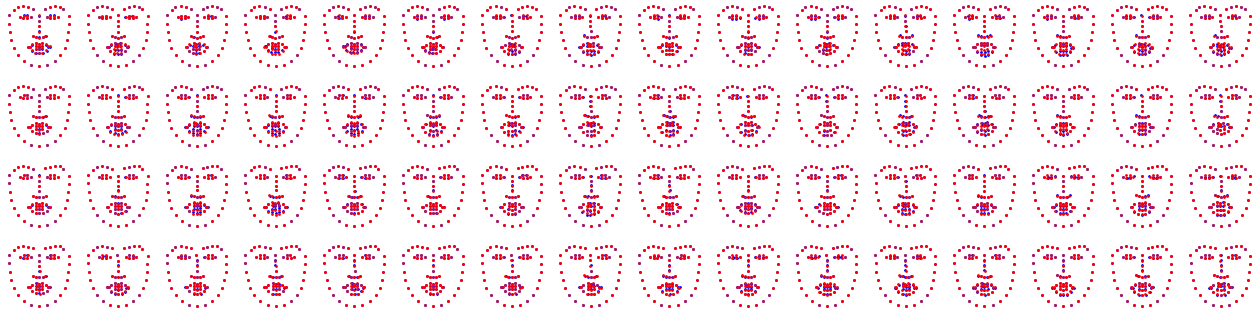
\includegraphics[width=15cm]{images/lrw_examples-landmark.png}
    \caption{Kết quả tạo sinh cột mốc gương mặt theo giọng nói trên tập LRW. Cột mốc gốc màu xanh, cột mộc tạo sinh màu đỏ}
\end{figure}
\end{frame}

\begin{frame}{Kết quả thí nghiệm}
Tạo sinh gương mặt trên tập GRID. Hầu hết video được tạo sinh trên tập test đều rõ ràng, có chuyển động miệng hợp lý
\begin{figure}[H]
    \centering
    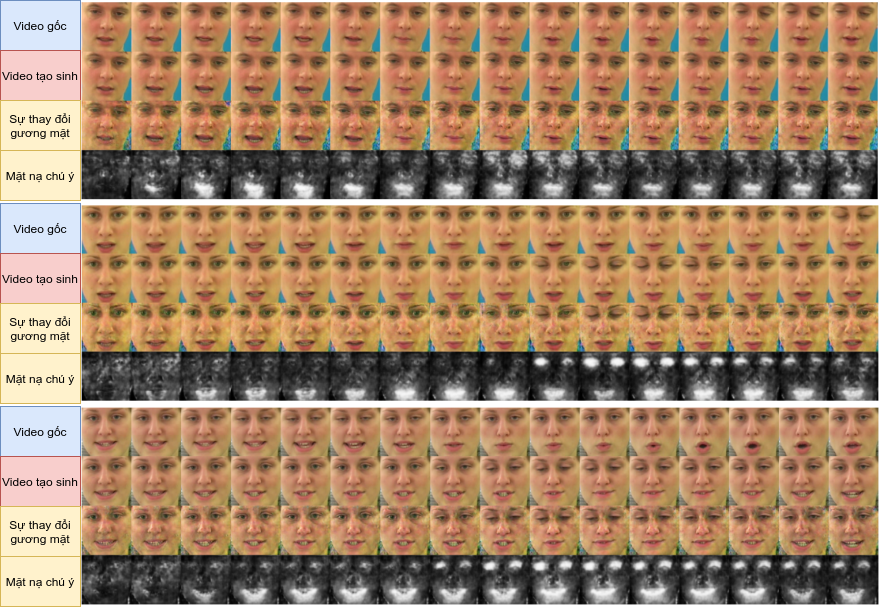
\includegraphics[width=15cm]{images/grid_examples-face.png}
    \caption{Kết quả tạo sinh gương mặt theo giọng nói trên tập GRID}
\end{figure}
\end{frame}

\begin{frame}{Kết quả thí nghiệm}
Tạo sinh gương mặt trên tập LRW. Hầu hết video được tạo sinh tốt khi hình ảnh đầu vào là hình chụp thẳng mặt. Chất lượng video bị suy giảm khi hình ảnh đầu vào được chụp ở các góc nghiêng
\begin{figure}[H]
    \centering
    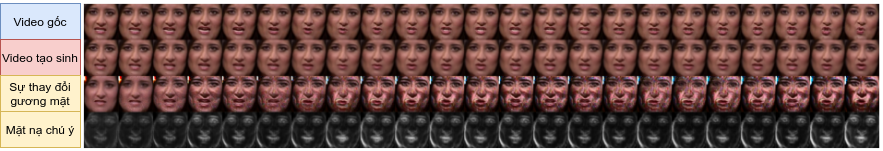
\includegraphics[width=15cm]{images/lrw_examples-face.png}
    \caption{Kết quả tạo sinh gương mặt theo giọng nói trên tập LRW}
\end{figure}
\end{frame}

\begin{frame}{Kết quả thí nghiệm}
\begin{table}[h]
    \centering
    \begin{tabular}{c | c | c | c | c}
    \hline 
    \multirow{2}{*}{\textbf{Phương pháp}} & \multicolumn{2}{c|}{\textbf{GRID}} & \multicolumn{2}{c}{\textbf{LRW}}\\
    \cline{2-5}
    & SSIM & CPBD & SSIM & CPBD\\
    \hline
    \textbf{Zakharov et al \cite{zakharov}} & 0.54 & 0.19 & 0.42 & 0.11 \\
    \textbf{Chung et al \cite{chung}} & 0.41 & \textbf{0.22} & 0.34 & \textbf{0.21} \\
    \textbf{Baseline (Chen et al) \cite{chen2019}} & 0.41 & 0.08 & 0.38 & 0.07 \\
    \hline
    \hline
    \textbf{Ours} & \textbf{0.72} & 0.12 & \textbf{0.54} & 0.06 \\
    \hline
    \end{tabular}
    \caption{So sánh với các mạng có cùng mục tiêu về độ đo SSIM và CPBD. Dữ liệu trong bảng được lấy từ bài khảo sát \cite{chen_survey}}
    \label{table:metrics_result}
\end{table}
Qua bảng trên ta thấy:
\begin{itemize}
    \item Độ tương đồng SSIM đã tăng đáng kể cho cả hai tập dữ liệu. Do đó, video tạo sinh có chuyển động giống video gốc hơn
    \item Độ nét tăng đối với tập GRID, tuy nhiên lại giảm trên tập LRW
\end{itemize}
\end{frame}

\begin{frame}{So sánh với mô hình gốc của Lele Chen}
    \begin{figure}[H]
        \centering
        \includegraphics[width=5cm]{images/comparision-grid.png}
        \caption{So sánh với mô hình của tác giả trên tập GRID. Bên trái là video được tạo sinh bởi mô hình mới, bên phải là của tác giả Lele Chen}
    \end{figure}
\end{frame}

\begin{frame}{So sánh với mô hình gốc của Lele Chen}
    \begin{figure}[H]
        \centering
        \includegraphics[width=10cm]{images/comparision-lrw.png}
        \caption{So sánh với mô hình của tác giả trên tập LRW. Bên trái là video được tạo sinh bởi mô hình mới, bên phải là của tác giả Lele Chen}
    \end{figure}
\end{frame}

\begin{frame}{So sánh với mô hình gốc của Lele Chen}
Về mặt cảm quan, ta thấy
\begin{itemize}
    \item Đối với thử nghiệm trên tập GRID, hình ảnh được tạo sinh bới mô hình mới có độ nét cao hơn
    \item Đối với thử nghiệm trên tập LRW, hình ảnh được tạo sinh bới mô hình mới có độ nét thấp hơn
    \item Trên video thực tế, thử nghiệm trên cả hai tập cho kết quả tạo sinh mượt mà hơn và khẩu hình miệng khớp hơn trên mô hình mới
\end{itemize}
Điều này phù hợp với kết quả khảo sát về độ đo SSIM và CPBD
\end{frame}
